\documentclass[a4paper, 14pt]{extarticle}

\usepackage{../latexDependencies/misc/preamble}

\geometry{a4paper}

% Название дисциплины
\newcommand{\subject}{Теория вероятности и математическая статистика} 

% Тип работы
% lab - для лабораторной работы 
% hw  - для домашней     работы
\newcommand{\task}{lab} 

% Номер работы
\newcommand{\taskNumber}{2} 

% Название работы
\newcommand{\taskNameOne}{Моделирование и обработка выборки } 
\newcommand{\taskNameTwo}{из дискретного закона распределения.} 

% Имя студента
\newcommand{\studentName}{Очкин Н.В.}

% Имя преподававателя
\newcommand{\teacherName}{Облакова Т.В.}

% Группа
\newcommand{\group}{ФН11-52Б}

% Вариант
\newcommand{\variant}{9}

\begin{document}

\graphicspath{ {../latexDependencies/images} } 
\normalsize

\newcommand{\printTask}{%
    \ifthenelse{\equal{\task}{lab}}{%
        лабораторной%
    }{%
        \ifthenelse{\equal{\task}{hw}}{%
            домашней%
        }{%
            Неизвестный тип задания%
        }%
    }%
}

\begin{titlepage}

    \begin{center}
        {\footnotesize \itshape Федеральное государственное бюджетное 
                       образовательное учреждение высшего образования}
    \end{center}

    \begin{minipage}[c]{0.1\textwidth}
        
\includegraphics[width=1.1\textwidth]{iconBMSTU}
    \end{minipage}
    \hfill
    \begin{minipage}[c]{0.9\textwidth}
        \centering
        \itshape
        \bfseries
        \small
        \guillemotleft Московский государственный технический университет \\
        имени Н.Э. Баумана\guillemotright \\
        (национальный исследовательский университет) \\
        (МГТУ им. Н.Э. Баумана) 
    \end{minipage}

    \vspace{0.5cm}
    \noindent\rule{\textwidth}{2pt} \\

    \noindent\uline{\textbf{ФАКУЛЬТЕТ} ФУНДАМЕНТАЛЬНЫЕ НАУКИ} \\
    \vspace{-5pt} \\
    \noindent\uline{\textbf{КАФЕДРА} ВЫЧИСЛИТЕЛЬНАЯ МАТЕМАТИКА И МАТЕМАТИЧЕСКАЯ} \\
    \vspace{-5pt} \\
    \noindent\uline{ФИЗИКА (ФН11)} \\
    \vspace{-5pt} \\
    \noindent\uline{\textbf{НАПРАВЛЕНИЕ ПОДГОТОВКИ} МАТЕМАТИКА И КОМПЬЮТЕРНЫЕ} \\
    \vspace{-5pt} \\
    \noindent\uline{НАУКИ (02.03.01)} \\

    \begin{center}
        \bfseries
        \textsc{О т ч е т} \\[10pt]
        по \printTask {} работе \textnumero {} \taskNumber
    \end{center}

    \vspace{10pt}

    \hspace{10pt} 
    \noindent \textbf{Название \printTask {} работы:} \par
    \vspace{5pt}
    \hspace{10pt} 
    \noindent \textbf{\uline{\taskNameOne}} \vspace{5pt} \\
    \null\hspace{31pt} 
    \textbf{\uline{\taskNameTwo}} \vspace{5pt} 

    \vspace{10pt}

    \begin{center}
        \bfseries
        Вариант \textnumero {} \variant
    \end{center}

    \vspace{20pt}

    \hspace{10pt} 
    \noindent \textbf{Дисциплина:} \par
    \vspace{10pt}
    \hspace{10pt} 
    \noindent {\large \subject}

    \vspace{10pt}

    \begin{flushright}
        \renewcommand{\arraystretch}{3}
        \begin{tabular}{r r r}
            \multicolumn{1}{l}{Студент группы \uline{\group}} & 
            $\quad \underset{\text{(Подпись, дата)}}{\underline{\hspace{3cm}}} \quad$ & 
            \multicolumn{1}{c}{$\underset{\text{(И.О. Фамилия)}}{\uline{\textbf{\studentName}}}$} \\

            \multicolumn{1}{l}{Преподаватель} & 
            $\quad \underset{\text{(Подпись, дата)}}{\underline{\hspace{3cm}}} \quad$ & 
            \multicolumn{1}{c}{$\underset{\text{(И.О. Фамилия)}}{\uline{\textbf{\teacherName}}}$} \\
        \end{tabular}
    \end{flushright}

    \vfill

    \begin{center}
        \small
        Москва, 2024
    \end{center}
\end{titlepage}


\newgeometry{left=25mm, right=25mm, top=20mm, bottom=20mm}

\graphicspath{ {../latexDependencies/images/LW2} }

\titleformat{\subsection}
  {\normalfont\normalsize\bfseries}{\thesubsection}{1em}{}

\thispagestyle{empty}

\null\newpage

\pagenumbering{arabic}
\setcounter{page}{1}

\setstretch{1}
\linespread{1.1}

\setlength{\parindent}{0pt}

\fontsize{12pt}{16pt}\selectfont

% --------------------------------------START--------------------------------------

\subsection*{Задание}

\begin{enumerate}
  \item Для заданных значений k, p и n смоделируйте выборку из биномиального закона распределения:
  \begin{equation*}
    P(\xi = j) = p_j = C_k^j p^j (1 - p)^{k - j}, j = \overline{0, k}.
  \end{equation*}
  \item Для полученной выборки постройте статистический ряд. Найдите эмпирическую функцию распределения $\tilde{F}_n(x)$.
  Постройте на одном рисунке графики $F(x)$ и $\tilde{F}_n(x)$. Вычислите статистику Колмогорова.
  \item Вычислите выборочное среднее и выборочную дисперсию и сравните с истинными значениями этих характеристик.
\end{enumerate}

\subsection*{Исходные данные}

\begin{equation*}
  k = 8, \qquad p = 0.7, \qquad n = 140
\end{equation*}

\subsection*{Порядок выполнения работы}

Найдем теоретический закон по формуле Бернулли(вектор P) и вычислим вектор
кумулятивных вероятностей u

\vspace{-10pt}

\begin{align*}
  & P =& \left[ 0.00007,\hspace{5pt} 0.00122,\hspace{5pt} 0.01   ,\hspace{5pt} 0.04668,\hspace{5pt} 0.13614,\hspace{5pt} 0.25412,\hspace{5pt} 0.29648,\hspace{5pt} 0.19765,\hspace{5pt} 0.05765\right] \\
  & u =& \left[0.00007,\hspace{5pt} 0.00129,\hspace{5pt} 0.01129,\hspace{5pt} 0.05797,\hspace{5pt} 0.1941 ,\hspace{5pt} 0.44823,\hspace{5pt} 0.7447 ,\hspace{5pt} 0.94235,\hspace{5pt} 1.     \right]
\end{align*}

Смоделируем вектор Y из n случайных чисел, 
по вектору Y разыграем вектор Х в соответствии со следующим алгоритмом:

\begin{center}
  \begin{minipage}{0.43\textwidth}
    \begin{tcolorbox}[colback=white!10, colframe=black, width=\textwidth]
      \begin{verbatim}
name: k
input: u, r
output: int

i = 0
for j in u length:
  if r is less than u_j:
      break
  i += 1

return i
      \end{verbatim}
    \end{tcolorbox}
  \end{minipage}
  \hspace*{0pt}
  \begin{minipage}{0.43\textwidth}
    \begin{gather*}
      X_j = k(u, Y_j) \\
      j = 0, \hspace{1pt} ..., \hspace{1pt} n - 1 
    \end{gather*}
  \end{minipage}
\end{center}

\newgeometry{left=25mm, right=25mm, top=10mm, bottom=20mm}

\begin{align*}
  & Y =& \left[0.22183838, 0.25624019, 0.05717201, \cdots,  0.13413202, 0.0200769 , 0.15263197 \right] \\
  & X =& \left[5, 5, 3, 6, 6, 3, 5, 6, 4, 7, 5, 5, \cdots, 7, 6, 4, 7, 7, 4, 3, 4 \right]
\end{align*}

Построим статистический ряд (см. Приложение) и запишем результат в виде таблицы:

\begin{table}[h!]
  \centering
  \renewcommand{\arraystretch}{1.4}
  \begin{adjustbox}{max width=0.6\textwidth}
    \begin{tabular}{|c|c|c|c|}
    \hline

    Значения  & \multirow{3}{*}{Частоты} & Относительные  & Накопленные \\
    случайной &                          & частоты        & частоты     \\
    величины  &                          &                &             \\

    \hline
    0 & 0 & 0 & 0 \\
    \hline
    1 & 1 & 0.00714286 & 0.00714286 \\
    \hline
    2 & 2 & 0.01428571 & 0.02142857 \\
    \hline
    3 & 8 & 0.05714286 & 0.07857143 \\
    \hline
    4 & 17 & 0.12142857 & 0.2 \\
    \hline
    5 & 37 & 0.26428571 & 0.46428571 \\
    \hline
    6 & 37 & 0.26428571 & 0.72857143 \\
    \hline
    7 & 31 & 0.22142857 & 0.95 \\
    \hline
    8 & 7 & 0.05 & 1 \\
    \hline
    \end{tabular}
  \end{adjustbox}
\end{table}

Вектор накопленных частот содержит ненулевые значения эмпирической функции распределения,
соответствующие значения теоретической функции распределения состовляют вектор u.
Для вычисления статистики Колмогорова:

\begin{equation*}
  D_n = \sup_{x \in \mathbb{R}} \left| \tilde{F}_n (x) - F (x) \right|
\end{equation*}

данные удобно свести в таблицу:

\begin{table}[h!]
  \centering
  \renewcommand{\arraystretch}{1.4}
  \begin{adjustbox}{max width=0.6\textwidth}
    \begin{tabular}{|c|c|c|c|}
    \hline

    \multirow{3}{*}{Интервал} & Эмпирическая  & Теоретическая  & Модуль   \\
                              & функция       & функция        & разности \\
                              & распределения & распределения  &          \\

    \hline
    $\left( -\infty, 0 \right]$ & 0 & 0 & 0 \\
    \hline
    $\left( 0, 1 \right]$ & 0 & 0.00007 & 0.00007 \\
    \hline
    $\left( 1, 2 \right]$ & 0.00714 & 0.00129 & 0.00585 \\
    \hline
    $\left( 2, 3 \right]$ & 0.02143 & 0.01129 & 0.01014 \\
    \hline
    $\left( 3, 4 \right]$ & 0.07857 & 0.05797 & 0.0206 \\
    \hline
    $\left( 4, 5 \right]$ & 0.2 & 0.1941 & 0.0059 \\
    \hline
    $\left( 5, 6 \right]$ & 0.46429 & 0.44823 & 0.01606 \\
    \hline
    $\left( 6, 7 \right]$ & 0.72857 & 0.7447 & 0.01613 \\
    \hline
    $\left( 7, 8 \right]$ & 0.95 & 0.94235 & 0.00765 \\
    \hline
    $\left( 8, +\infty \right)$ & 1 & 1 & 0 \\
    \hline
    \end{tabular}
  \end{adjustbox}
\end{table}

\newgeometry{left=25mm, right=25mm, top=20mm, bottom=20mm}

Из данных таблицы следует, что максимальное различие теоретической и 
эмпирической функций распределения наблюдается на  полуинтервале $\left( 3, 4 \right]$.
Заметим  также,  что  значение  статистики Колмогорова $D_{140} = 0.0206$ невелико, что 
говорит о приемлемом результате моделирования.\\

Изобразим совмещенные графики эмпирической и теоретической функций распределения:

\begin{center}
  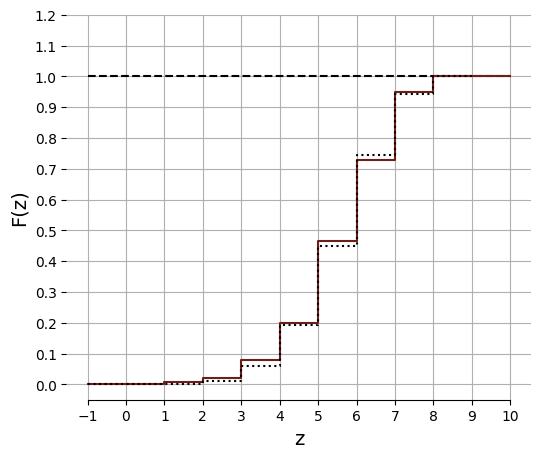
\includegraphics[width=0.8\textwidth]{1}
\end{center}

где красной линией отмечен график эмпирической функции распределения; \\
черной пунктирной - теоретической. \\

Выполнение  работы  завершим  вычислением  эмпирических 
и теоретических характеристик.

\begin{align*}
  & \text{Выборочное среднее} &=\hspace{10pt}& m \mu &=\hspace{10pt}& \cfrac{1}{n} \cdot \sum_{k=0}^{n} X_k &=\hspace{10pt}& 5.55 \\ 
  & \text{Выборочная дисперсия} &=\hspace{10pt}& S^2 &=\hspace{10pt}& \cfrac{1}{n - 1} \cdot \sum_{k=0}^{n} (X_k - m \mu)^2 &=\hspace{10pt}& 1.90396 \\ 
  & \text{Математическое ожидание} &=\hspace{10pt}& m &=\hspace{10pt}& \sum_{i=0}^{n} \left(i \cdot P_i \right) &=\hspace{10pt}& 5.6 \\ 
  & \text{Дисперсия} &=\hspace{10pt}& D &=\hspace{10pt}& \sum_{i=0}^{n} \left[ \left( i - m \right)^2 \cdot P_i \right] &=\hspace{10pt}& 1.68 
\end{align*}

Поскольку абсолютная величина разности математического ожидания 
и выборочного среднего мала, а отношение выборочной 
дисперсии к ее теоретическому значению близко к единице, то 
результаты моделирования можно признать удовлетворительными.

\subsection*{Итог}

В ходе проделанной лабораторной работы было проведено моделирование 
и обработка выборки из дискретного закона распределения. Для полученной 
выборки построен статистический ряд и эмпирическая функция распределения, 
вычислена статистика Колмогорова. На основании значений выборочного среднего 
и выборочной дисперсии был сделан вывод о степени качества моделирующей дискретный 
закон выборки.

% --------------------------------------CODE---------------------------------------

\subsection*{Приложение}

Программный код, с помощью которого была выполнена данная лабораторная работа.\\

\vspace{15pt}

{\footnotesize
\noindent \textbf{Примечание}.\\

\vspace{-10pt}

\noindent Так как отчет был написан с использованием дистрибутива TeX и 
следующий код был отформатирован с использованием окружения \textsc{lstlisting}, 
в некоторых местах текст, написанный на русском языке, может иметь проблемы 
с выравниванием, пробелами, шрифтом и т.д. Это связано с тем, что библиотека 
\textsc{listings}, из которой мы берем окружение для форматирования кода, 
плохо работает с Unicode.
}

\vspace{20pt}

\setstretch{1}

\lstdefinestyle{mystyle}{
    basicstyle=\ttfamily\footnotesize,
    keywordstyle=\color{blue},
    stringstyle=\color{red},
    commentstyle=\color{green!50!black},
    showstringspaces=false
}

% Set the style for Python code
\lstset{style=mystyle, language=Python, extendedchars=\true}

\begin{lstlisting}
import numpy as np
import math
import matplotlib.pyplot as plt

np.set_printoptions(suppress=True)

PRECISION = 5

k = 8   # Количество испытаний
p = 0.7 # Вероятность успеха в одном испытании
n = 140 # Объем выборки

probs = [] # Вероятности

for j in range(k + 1):
    pj = math.comb(k, j) * p**j * (1 - p)**(k - j) # формула Бернулли
    probs.append(pj)

np.round(np.array(probs), PRECISION)

kumProbs = [sum(probs[:(i + 1)]) for i in range(k + 1)] # Кумулятивные вероятности

np.round(np.array(kumProbs), PRECISION)

Y = np.random.rand(n) # n случайных величин
Y

# По вектору Y разыгрываем вектор X в соответствии с алгоритмом
def k_func(u, r):
    i: int = 0
    for j in range(len(u)):
        if r < u[j]:
            break
        i += 1
    return i

X = []

for Yj in Y:
    X.append(k_func(kumProbs, Yj))

print(X)

# Строим статистический ряд
def findFreq(data, k):
    values = np.arange(k + 1)
    counting = {}
    for value in values:
        counting[value] = 0

    for el in data:
        counting[el] += 1
    
    return [counting[el] for el in values]

values  = np.arange(k + 1)
freq    = findFreq(X, k)
relFreq = np.array(freq) / n
kumFreq = np.array([sum(relFreq[:(i + 1)]) for i in range(len(relFreq))])

print(f'Значения случайной величины: {values}')
print(f'Частоты:                     {freq}')
print(f'Относительные частоты:       {relFreq}')
print(f'Накопленные частоты:         {kumFreq}')

def CDF(z, values, kumFreq):
    if z <= values[0]:
        return 0
    
    if len(values) > 1:
        for i in range(1, len(values)):
            prev = values[i - 1]
            curr = values[i]

            if prev < z <= curr:
                return kumFreq[i - 1]

    if z > values[-1]:
        return 1

        def buildCDF(data, 
        cdf, values, kumFreq, 
        theoretical_cdf_y_values):

RED   = '#6F1D1B'

# Define font sizes
SIZE_DEFAULT = 14
SIZE_LARGE   = 16
SIZE_TICKS   = 10
plt.rc("font", weight="normal")          # controls default font
plt.rc("font", size=SIZE_DEFAULT)        # controls default text sizes
plt.rc("axes", titlesize=SIZE_LARGE)     # fontsize of the axes title
plt.rc("axes", labelsize=SIZE_DEFAULT)   # fontsize of the x and y labels
plt.rc("xtick", labelsize=SIZE_DEFAULT)  # fontsize of the tick labels
plt.rc("ytick", labelsize=SIZE_DEFAULT)  # fontsize of the tick labels

_, ax = plt.subplots(
   figsize=(6, 5)
)

# Generate a range of x values
x_values = np.linspace(-1, np.max(data) + np.min(data) + 1, 100)

# Evaluate the function for each x value (empirical)
cdf_y_values = [cdf(x, values, kumFreq) for x in x_values]

xticks = [i for i in range(-1, int(np.max(data) + np.min(data)) + 1 + 1)]
yticks = np.arange(0, 1.2 + 0.1, 0.1)

# Hide the all but the bottom spines (axis lines)
ax.spines["right"].set_visible(False)
ax.spines["left"].set_visible(False)
ax.spines["top"].set_visible(False)

# Only show ticks on the left and bottom spines
ax.yaxis.set_ticks_position("left")
ax.xaxis.set_ticks_position("bottom")
ax.spines["bottom"].set_bounds(min(xticks), max(xticks))

# plot y = 1 line
plt.plot(x_values, np.full_like(x_values, 1), label='y = 1', linestyle='--', 
                                                             color='black')

# Plot cdf(x) (empirical)
plt.step(x_values, cdf_y_values, label='empirical(x)', color=RED)

# Plot the theoretical distribution function
x_values = np.arange(-1, k + 2)
plt.step(x_values, theoretical_cdf_y_values, label='theoretical(x)', 
                   color='black', linestyle='dotted')

# axis names
plt.xlabel('z')
plt.ylabel('F(z)')

plt.xticks(xticks)
plt.yticks(yticks)

# Adjust the font size of the tick labels
plt.tick_params(axis='both', which='major', labelsize=SIZE_TICKS)

plt.grid(True)

plt.show()

kumProbs = [0] + [0] + kumProbs
buildCDF(X, 
         CDF, values, kumFreq, # эмпирическая
         kumProbs)             # теоретическая

empirVals = []
theoretVals = []
diffs = []
print(f'значение: ', end='')
for i in range(0, k + 2):
    print(f'({i-1}, {i}]',end=', ')
    empirVal   = CDF(i, values, kumFreq)
    theoretVal = kumProbs[i + 1]
    diff = abs(empirVal - theoretVal)

    empirVals.append(empirVal)
    theoretVals.append(theoretVal)
    diffs.append(diff)

print(f'\n эмпир функция распр: {np.round(np.array(empirVals), PRECISION)}')
print(f'теор функция распр:  {np.round(np.array(theoretVals), PRECISION)}')
print(f'модуль разности:     {np.round(np.array(diffs), PRECISION)}')

D = max(diffs)
print(f'\nD = {D}')

# эмпирическая

# выборочное среднее
overlineX = np.round((1 / n) * np.sum(X), PRECISION)
m1 = np.mean(X)

# выборочная дисперсия
S2 = np.round(1 / (n - 1) * np.sum((X - overlineX)**2), PRECISION)

print(f'выборочное среднее: {overlineX} ({m1})')
print(f'выборочная дисперсия: {S2}')

# теоретическая

# мат ожидание
m = sum([i * probs[i] for i in range(k + 1)])

# дисперсия
d = sum([(i - m)**2 * probs[i] for i in range(k + 1)])

print(f'мат ожидание: {m}')
print(f'дисперсия: {d}')
\end{lstlisting}

\end{document}
